\documentclass[11pt]{article}
\usepackage[T1]{fontenc}
\usepackage{fourier}
\usepackage{setspace}
\usepackage[protrusion=true,expansion=true]{microtype}	
\usepackage{amsmath,amsfonts,amsthm} % Math packages
\usepackage[pdftex]{graphicx}	
\usepackage{subfigure}
\usepackage{url}
\usepackage{caption}
\usepackage{float}
\usepackage{fancyhdr}
\usepackage{geometry}
\newcommand{\argmin}{\arg\!\min}
\usepackage{amssymb}
\usepackage{amsmath}
\usepackage{wrapfig}
\usepackage{textcomp}
\usepackage{multirow}
\usepackage{boldline}
\usepackage{upgreek}
\usepackage{array}
\usepackage[table]{xcolor}
\usepackage{graphicx}
\usepackage[utf8]{inputenc}
\usepackage[inline]{enumitem}
\usepackage{chngcntr}
\usepackage{verbatim}
\newcommand\bmmax{2}
\usepackage{bm}
\usepackage{siunitx}
\usepackage{eurosym}
\usepackage{booktabs}
\usepackage{fancyhdr}
\usepackage{titlesec}
\usepackage{textgreek}
\usepackage{fancyhdr}
\graphicspath{ {graph/} }
\usepackage{geometry}

\geometry{left=2cm,right=2cm,top=2cm,bottom=2cm}
\pagestyle{fancy}
\fancyhf{}

\counterwithin{table}{section}
\counterwithin{figure}{section}
\counterwithin{equation}{section}

\makeatletter
% This command ignores the optional argument for itemize and enumerate lists
\newcommand{\inlineitem}[1][]{%
\ifnum\enit@type=\tw@
    {\descriptionlabel{#1}}
  \hspace{\labelsep}
\else
  \ifnum\enit@type=\z@
       \refstepcounter{\@listctr}\fi
    \quad\@itemlabel\hspace{\labelsep}
\fi}
\makeatother

\usepackage{helvet}
\renewcommand{\familydefault}{\sfdefault} 

\renewcommand{\rmdefault}{phv} 
 \renewcommand{\sfdefault}{phv} 
\renewcommand{\headrulewidth}{0.5pt}



\begin{document}
\doublespacing
\pagenumbering{arabic}


%%%%%%%%%%%%%%%%%%%%%%%%%%%%%%%%%%%%%%%%%%%%%%%%%%%%%%%%%%%%%%%%%%%%%%%%%%%%%%%%%%%%%%%%%%%%%%%%%%%%%%%%%%%%%%%%%%%%%%%%%%%%%%%%%%%%%%%%%%%%%%%%%%%%%%%%%%%%%%%%%%%%%%%%%%%%%%%%%%%%%%%%%%%%%%%%%%%%%%%%%%%%%%%%%%%%%%%%%%%%%%%%%%%%%%%%%%%%%%%%

\begin{titlepage}

\newcommand{\HRule}{\rule{\linewidth}{0.5mm}} % Defines a new command for the horizontal lines, change thickness here

\center % Center everything on the page
 
%----------------------------------------------------------------------------------------
% HEADING SECTIONS
%----------------------------------------------------------------------------------------

\includegraphics[width=0.2\linewidth]{Graph/Oxford-University-Logo.png}\\[1cm]

\textsc{\Large Department of Engineering Science}\\[0.5cm] % Major heading such as course name
\textsc{\large Reading Note}\\[0.5cm] % Minor heading such as course title
{\large \today}
\HRule \\[0.4cm]
{ \huge \bfseries Information Theory, Inference, and Learning Algorithm}\\[0.4cm] % Title of your document
\HRule \\[1.5cm]

\begin{minipage}{0.4\textwidth}
\begin{flushleft} \large
\emph{Author:}
\\Shuqi \textsc{Zhang}
\end{flushleft}
\end{minipage}
~
\begin{minipage}{0.4\textwidth}
\begin{flushright} \large
\emph{Supervisors:} \\
Prof. Michael \textsc{Osborne} % Supervisor's Name
\end{flushright}
\end{minipage}\\[1cm]



\end{titlepage}
%%%%%%%%%%%%%%%%%%%%%%%%%%%%%%%%%%%%%%%%%%%%%%%%%%%%%%%%%%%%%%%%%%%%%%%%%%%%%%%%%%%%%%%%%%%%%%%%%%%%%%%%%%%%%%%%%%%%%%%%%%%%%%%%%%%%%%%%%%%%%%%%%%%%%%%%%%%%%%%%%%%%%%%%%%%%%%%%%%%%%%%%%%%%%%%%%%%%%%%%%%%%%%%%%%%%%%%%%%%%%%%%%%%%%%%%%%%%%%%%

This pdf is a personal reading note for the book "Information Theory, Inference, and Learning Algorithm". The words in black are mainly from the book itself, while \textbf{\textcolor{red}{the words in red are personal understanding on the contents and futher explaination in my own words.} }

\newpage


\tableofcontents
%\setlength{\cftsubsecnumwidth}{4em}% Set length of number width in ToC for \subsection
%\makeatother

\newpage

\lhead{Shuqi Zhang}
\rhead{David J.C. MacKay: Information theory, Inference, and Learning Algorithms}

\thispagestyle{fancy} 
\clearpage






\section{Probability, Entropy, and Inference}

\begin{description}
  \item[Probability] To describe \textit{degress of belief} in propositions that do not involve random variables.
\end{description}

You cannot do inference without making asumptions.

\begin{description}
  \item[Bayesian method] Bayesians also use probabilities to describe inferences.

  \item[non-Bayesian method] probabilities are allowed to describe only random variables.
\end{description}

Probability calculations often fall into one of two categories \textbf{forward probability} and \textbf{inverse probability}.

\begin{description}
  \item[forward probability] \textit{generative model} that describes a process that is assumed to give rise to some data, and the data allow people to compute the probability distribution or expectation of some quantity.

  \item[inverse probability] \textit{generative model} that describes a process that is assumed to give rise to some data, however, we compute the conditional probability of one or more of the unobserved variables in the process, given the observed variables. \textbf{Bayesian theorem is required.}
\end{description}

\subsection{Terminologt of inverse probability}

Inverse probability is the one applied \textbf{Bayesian theorem}.

\begin{equation}
P(u|n_B, N) = \frac{P(u)P(n_B|u, N)}{P(n_B|N)}
\end{equation}

\begin{description}
  \item[prior] the marginal probability $P(u)$ is the \textit{prior} probability of u.

  \item[likelihood] $P(n_B|u, N)$ is called the \textit{likelihood} of u. For fixed $u$, $P(n_B|u, N)$ defines a probability over $n_B$. For fixed $n_B$, $P(n_B|u, N)$ defines the likelihood of $u$. In predition, $n_B$ is like the data set which is fixed, and $u$ is the model, therefore, $P(n_B|u, N)$ is the likelihood and it is the outcomes of the believed model. \textit{Always say "the likelihood of the parameters". The likelihood function is not a probability distribution.}

  \item[posterior] $P(u|n_B, N)$ is called the \textit{posterior} probability of $u$ given $n_B$.

  \item[evidence] the normalizing constant $P(n_B|N)$
\end{description}

\begin{equation}
posterior = \frac{likelihood \times prior}{evidence}
\end{equation}

\newpage

\section{An Example Inference Task: Clustering}
Regularity is to put a set of objects into groups that are similar to each other. The operation of grouping things togther is called \textit{clustering}. If the \textit{cluster} is further sub-divided into \textit{sub-clusters}, it is called \textit{hierarchical clustring}.\\

The motivations for clustering:

\paragraph{Reason 1}
  A good clustering has predictive power, helping people to better allocate their resources. The underlying cluster labels are meaningful, will lead to a more efficient description of our data, and will help people choose better actions. The information content of the data, $log\frac{1}{P({\mathrm{x}})}$.
\paragraph{Reason 2} Clusters can be a useful aid to communication because they allow lossy compression. Clusters can help people identify an object as they contain sufficient information.

\textbf{Vector quantizer} in terms of an \textit{assignment rule} $x \rightarrow k(x)$ for assigning datapoints $x$ to one of $K$ codenames, and a \textit{reconstruction rule} $k \rightarrow m^{(k)}$. The aim is to choose the function $k(x)$ and $m^(k)$ so as to minimize the \textit{expected distortion} for the reconstruction, which might be defined to be

\begin{equation}
D = \sum_x P(\mathrm{x})\frac{1}{2}[\mathrm{m^{kx}}-\mathrm{x}]^2  
\end{equation}

So the goal is to minimize $D$.

\paragraph{Reason 3}
  Failures of the cluster model may highlight interesting objects that deserve special attention. If something goes wrong in a vector quantizer, it is easier for people to figure out the reasons behind due to clusters.
\paragraph{Reason 4}
  Clustering algorithms may serve as models of learning processes in neural systems. The K-means algorithm is an example of a \textit{competitive learning} algorithm. The algorithm works by having the $K$ clusters compete with each other for the right to own the data points.

\subsection{K-means clustering}
An algorithm for putting \textit{N} data points in an \textit{I}-dimensional space into \textit{K} clusters. Each cluster is parameterized by a vector $m^k$ which is its mean. The data points are denoted by {$x^n$} and $n$ means $N$ data points. Each vector $x$ has $I$ components $x_i$, as it is $I$-dimension.

The K-means clustering algorithm:
\paragraph{Initialization.}
  Set $K$ means ${m^k}$ to random values.
\paragraph{Assignment step.}
 Each data points $n$ is assigned to the nearest mean. We denote our guess for the cluster $k^n$ that the point $x^n$ belongs to by $\hat{k}^n$.
  \begin{equation}
  \hat{k}^n = \operatorname*{argmin}_x \{d(m^k,x^n)\}
  \label{K}
  \end{equation}

  \textcolor{red}{The equation \ref{K} about is trying to minimize the distance between the assumed means and the actual data points.}

  \begin{equation}
    responsibilities,\ r^n_k=
    \begin{cases}
      1, & \text{if}\ \hat{k}^n = k. \\
      0, & \text{if}\ \hat{k}^n \neq k.
    \end{cases}
  \end{equation}

  \textcolor{red}{If mean $k$ is the closest mean to datapoint, the responsibility is equal to 1, therefore $\hat{k}^n$ is equal to $k$. It means that the assumed cluster $\hat{k}^n$ is actually the correct cluster. However, if not, then the responsibility is zero. If $r$ is 1, then the corresponding $\hat{k}^n$ is the winning ${k}$.}

\paragraph{Update step.}
  $m^k$ is updated to match the means of the data points.

  \begin{equation}
    m^k = \frac{\sum_n r^n_k x^n}{R^k}
  \label{update}
  \end{equation}

  where $R^k$ is the total responsibility of mean $k$, \textcolor{red}{and the sum is for each data point \textquotesingle s responsibility and the data value for to corresponding cluster.}

  \begin{equation}
    R^k = \sum_n r^n_k 
  \end{equation}

\paragraph{Repeat the assignment step and update step.}
  Keep repeating the loop untill the assginment step gives the mean is the cloest one.

  \textcolor{red}{Mean $m$ has been assigned with a random value, and the minimum $\hat{k}$ has been found for each $k$ \textit{$k^n$ means that the $k$ which is the cluster has the same number as the data points $n$}. As the original $m$ is a random value, it is updated by the equation \ref{update}.}

\paragraph{\textbf{\textcolor{red}{Personal understanding of K-means algorithm}}}
  \textcolor{red}{There are two inputs in the K-means algorithm: $K \rightarrow$ number of cluster; $x_i \rightarrow$ represents the set of points with $i$ ranges from $1$ to $n$. At the beginning of the process, centroids $C_j$, where $i$ is equal to the number of clusters, are placed at random locations. For each data points $x_i$, $argmin$ has been used to compare the distance between each data point and each centroid, generating the nearest centroid $C_j$. The data point $x_i$ is assgined to the cluster $C_j$ individually. For example, if there are two centroids, all the data points have been assigned to two clusters based on their distances. After assignment, the position or value of clusters will be recomputed according to the positions or values of the data points belong to them. Equation \ref{update} shows that the update only related to the points belong to the cluster as responsibility, $r$, needs to be $1$ to be meaningful in the calculation. By taking the average of the positions of cluster \textquotesingle s data points, the new cluster \textquotesingle s position is computed. The loop of assigment of data points to clusters and update of clusters keeps running untill the assigment does not change.}
\textcolor{red}
{
\begin{enumerate}
  \item Data points have been assigned to clusters.
  \item Clusters have been updated based on their data points.
  \item Data points are assigned again based on the updated clusters.
  \item Clusters are updated as the data points \textquotesingle assigments have been changed.
  \item Keep assigning and updating untill assigment does not change.
  \item The number of iterations is related to the clusters \textquotesingle initial locations.
\end{enumerate}
}

The algorithm is based on distance between clustes and data points (distance between the means and the data points), so the algorithm may igore the general patterns, ending up with some points may be incorrectly assigned to the wrong clusters. \textit{(refer to the book Figure 20.5 and Figure 20.6)} The K-means algorithm has no representation of the weight or breadth of each cluster. Consequently, data points that actually belong to the broad cluster are incorrectly assigned to the narrow cluster. \textcolor{red}{\textbf{The K-means algorithm has no way of representing the size or shape of a cluster.} This algoritm is rather too hard as all points assigned to a cluster are equals in that cluster. However, some points are closer to the centroid while some are placed near the border between two or more clusters should play a partial role in determining the locations of all the clusters that they could plausibly be assigned to \textit{(further determination befer jumping into conclusion recklessly)}.}

\subsection{Soft K-means clustering}
$\beta$ is inputted for people to term the \textit{stiffness}. The stiffness $\beta$ is an inverse-length-squared, so it can be associated a lengthscale, $\theta \equiv 1 / \sqrt{\beta}$.

\paragraph{Assignment step.}
  Each data point $x^n$ is given a soft 'degree of assignment' to each of the means \textit{(each of the centroids)}. We call the degree to which $x^n$ is assigned to cluster $k$ the responsibility $r^n_k$. The $\beta$ is considered into the calculation of responsibility, $r$.

\begin{equation}
  r_k^n = \frac{exp(-\beta d (m^k, x^n))}{\sum_{k'}exp(-\beta d(m^{k'},x^n))}
\end{equation}

The sum of the $K$ responsibilities for the $n$th point is 1.

\paragraph{Updated step.}
  The clusters \textquotesingle positions are updated by the same method as the normal K-mean algorithm.

  \begin{equation}
    m^k = \frac{\sum_n r^n_k x^n}{R^k}
  \label{update}
  \end{equation}

  where $R^k$ is the total responsibility of mean $k$, \textcolor{red}{and the sum is for each data point \textquotesingle s responsibility and the data value for to corresponding cluster.}

  \begin{equation}
    R^k = \sum_n r^n_k 
  \end{equation}

\textcolor{red}{The responsibility, $r^n_k$, can take values between $0$ and $1$, therefore, the points assigned to a specific cluster are not equal. \textbf{Therefore, weights have added to the data points assigned to a cluster. The points closer to the centroid are $1$ and the points futher or in between are from $1$ to $0$, but still assigned to the same cluster. When the centroid is updated, different points have different weights in the new postion calculation, so the new cluster can be placed more cenral to the correct points.}}


\newpage

\section{Exact Inference by Complete Enumeration}
The phenomenon, that one of the possible causes ($b=1$) of some data (another action, $a$) becomes \textit{less} probable when another of the causes ($c = 1$) becomes \textit{more} probable, even though those two causes are independent varibales $a$ \textit{prior}, is known as \textit{explaining away}.

\textcolor{red}{This kind of problems is solved byenumerating all hypotheses about the variables ($b,c$), finding their posterior probabilities, and marginalizing to obtain the required inferences about one, ($b or c$) over the other, ($c or b$).}

\subsection{Exact inference for continuous hypothesis spaces}
Many of the hypothesis psaces we will consider are naturally thought of as contiuous. For example, standard deviation of a Gaussian $\mu, \delta$ live in a continuous two-dimensional space. In computer implementation, such continuous spaces will necessaryily be discretized or be enumerated at a grid of parameter values.

\paragraph{A two-parameter model}
The one-dimensional Gaussian distribution is parameterized by a mean $\mu$ and a standard deviation $\delta$:

\begin{equation}
  P(x | \mu, \delta) \equiv Normal(x; \mu, \delta^2)
\end{equation}

\begin{figure}[H]
\centering
 \frame{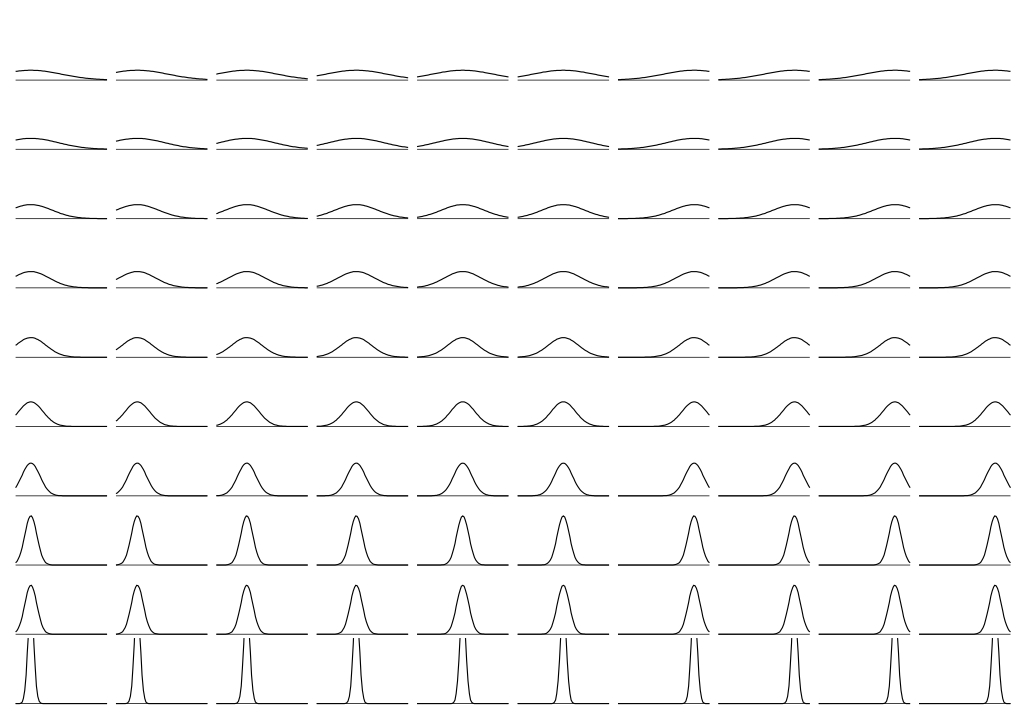
\includegraphics[width=0.64\linewidth]{Graph/enumeration1.png}}
 \caption{Enumeration of an entire (discretized) hypothesis space for one Gaussian with parameters $\mu$ (horizontal axis) and $\delta$ (vertical).}
 \label{fig:enumeration1}
\end{figure}

Figure \ref{fig:enumeration1} shows  that hypotheses are evenly spaced in a ten by ten square grid covering ten values of $\mu$ nd ten values of $\delta$. The inference of $\mu$ and $\delta$ are examined given data points $x_n$ for $n$ ranging for $1$ to $N$.\textcolor{red}{The model is discretized in two-dimension and the inference is examnied by the data points.} The data points can be placed in the inference to find the maximum likelihood. The line thikcness, figure \ref{fig:enumeration3}, can be used to encode the value of the likelihood and the sub-hypotheses with likelihood smaller than $e^{-8}$ times the maximum likelihood are deleted.


\begin{figure}[ht]
\begin{minipage}[b]{0.45\linewidth}
\centering
  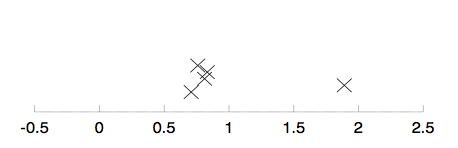
\includegraphics[width=\textwidth]{Graph/enumeration2.png}
  \caption{Five datapoints.}
  \label{fig:datapoints1}
\end{minipage}
\hspace{0.5cm}
\begin{minipage}[b]{0.45\linewidth}
\centering
  \frame{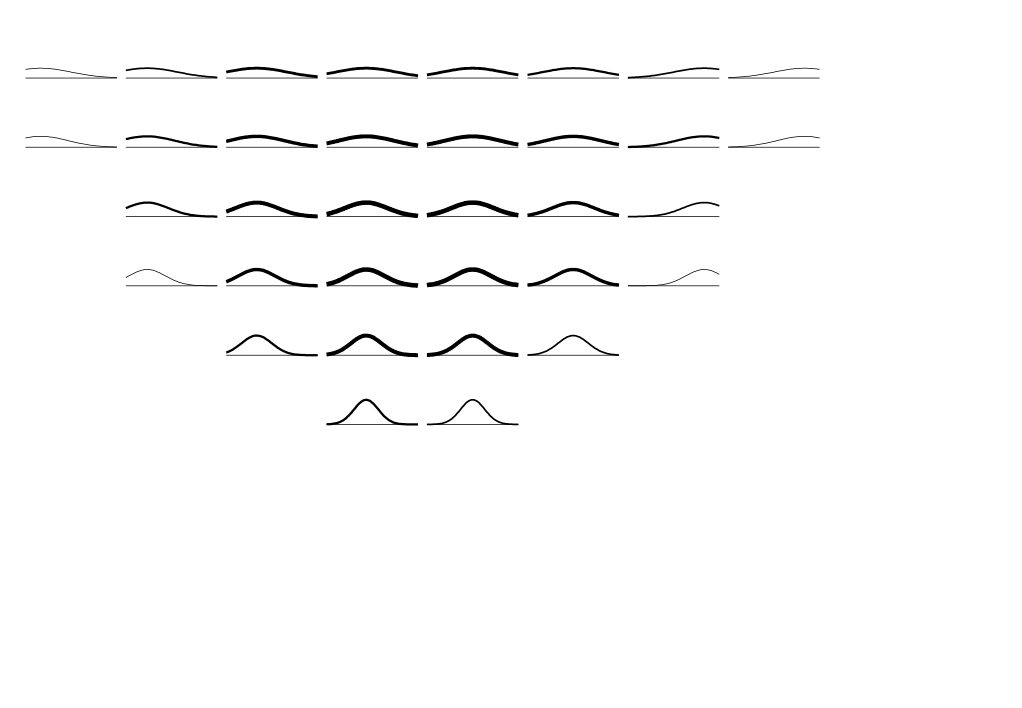
\includegraphics[width=\textwidth]{Graph/enumeration3.png}}
  \caption{Likelihood function from figure \ref{fig:enumeration1}, given the data of figure \ref{fig:datapoints1}, represented by line thickness.}
  \label{fig:enumeration3}
\end{minipage}
\end{figure}


\paragraph{A five-parameter mixture model}
A mixture of two Gaussian to represent the points in figure \ref{fig:datapoints1}

\begin{equation}
  P(x | \mu_1, \delta_1, \pi_1, \mu_2, \delta_2, \pi_2) \equiv Normal(x; \mu_1, \delta^2_1, \pi_1, \mu_2, \delta^2_2, \pi_2)
\end{equation}

Where $\pi$ is weighting between two Gaussian distributions. Because $\pi_1 + \pi_2 = 1$, it only represents one dimension. There are five dimensions in total, $\mu_1, \delta_1, \mu_2, \delta_2, \pi$.

\begin{figure}[H]
\centering
 \frame{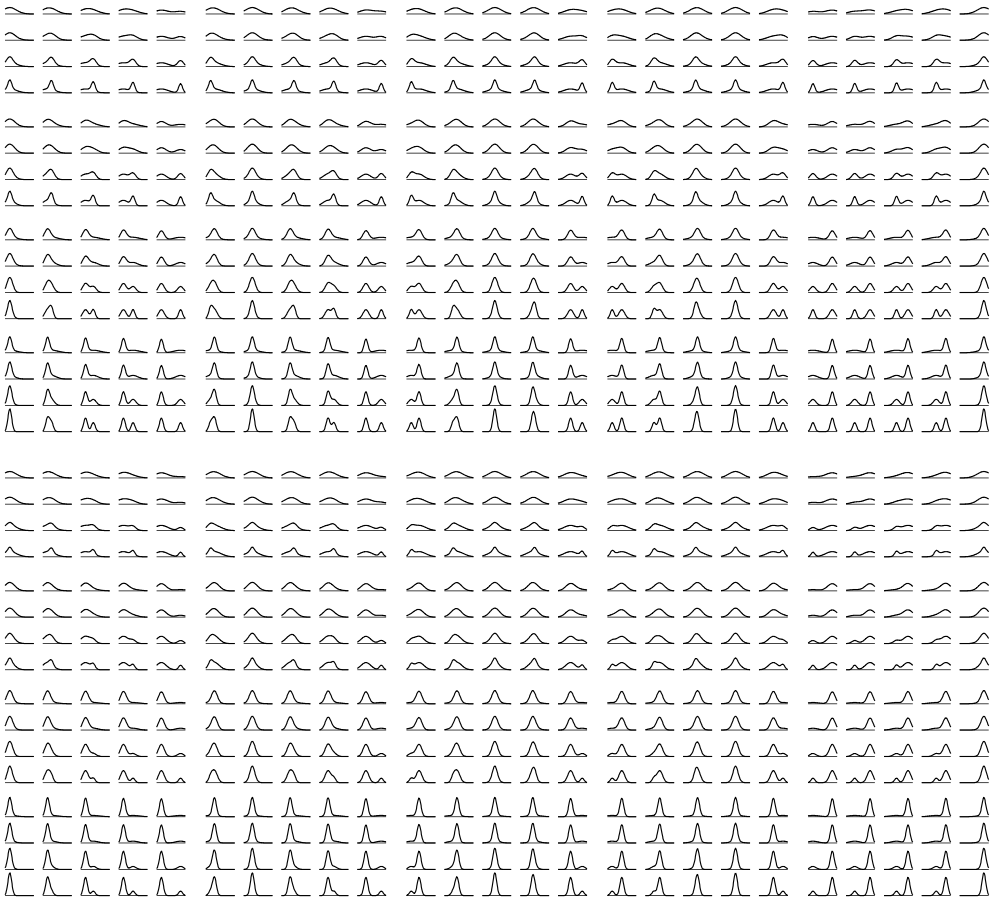
\includegraphics[width=0.5\linewidth]{Graph/enumeration4.png}}
 \caption{Enumeration of the entire (discretized) hypothesis space for a mixture of two Gaussians. Weight of the mixture components is $\pi_1, \pi_2 = 0.6, 0.4$ in the top half and 0.8, 0.2 in the bottom half. Means $\mu_1 and \mu_2$ vary horizontally, and standard deviations $\delta_1 and \delta_2$ vary vertically.}
 \label{fig:enumeration4}
\end{figure}

\textcolor{red}{For the first row, there are five blocks. $\mu_2$ changes evenly in horizontal direction, while $\delta_2 and \pi$ are fixed. Within each block, $\mu_1$ changes evenly in horizontal direction and $\delta_1$ changes evenly in vertical direction. Same rule applies to whole figure \ref{fig:enumeration4}.}

\begin{figure}[H]
\centering
 \frame{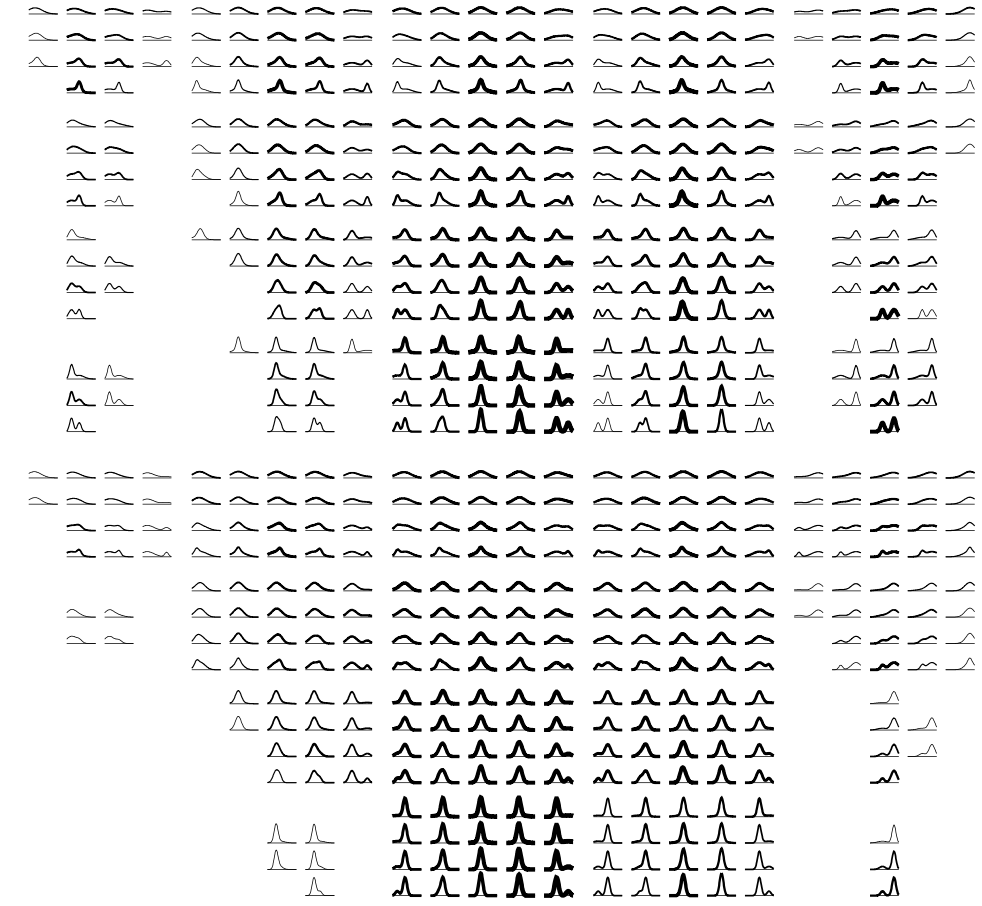
\includegraphics[width=0.5\linewidth]{Graph/enumeration5.png}}
 \caption{Inferring a mixture of two Gaussians. Likelihood function, given the data points, represented by line thikcness.}
 \label{fig:enumeration5}
\end{figure}

Models can be compared by the models \textquotesingle posterior probabilities \textit{(found by evaluating the marginal likelihood or evidence for each model $H, P({x}|H)$)}. \textcolor{red}{It is same as finding marginal over one parameter and compare the posterior of the model over that parameter. Moreover, normally, a grid of at least $10^k$ is required for the enumeration way to solve $K$ parameters model. Completing enumeration is rarely a feasible computational strategy due to the exponential growth of computation.}






\newpage

\section{Maximum Likelihood and Clustering}
\textcolor{red}{Comparing to enumerate all hypotheses, homing in on one good hypothesis that fits the data well saves a lot of time. It is supported by the maximum likelihood method.} It is easier to solve with the \textit{logarithm} of the likelihood as likelihoods multiple; log likelihoods add. 

\subsection{Maximum likelihood for one Gaussian}
For data ${x_n}^N_{n=1}$, the log likelihood is:

\begin{equation}
  \mathrm{ln}[P((x_n)^N_{n=1}|\mu,\delta)] = -N \mathrm{ln}(\sqrt{2\pi}) - \sum_n \frac{(x_n - \mu)^2}{2 \mu^2}
  \label{equation:maximum1}
\end{equation}

Where $\mu$ is the maximum likelihood meand of the Gaussian. The log can be xpressed in terms of two functions of the data, the sample mean, $\bar{x}$,

\begin{equation}
  \bar{x} \equiv \sum_{n=1}^N \frac{x_n}{N},
  \label{equation:maximum2}
\end{equation}

and the sum of deviations

\begin{equation}
  S \equiv  \sum_n (x_n - \bar{x})^2 :
  \label{equation:maximum3}
\end{equation}

\begin{equation}
  \mathrm{ln}[P((x_n)^N_{n=1}|\mu,\delta)] = -N \mathrm{ln}(\sqrt{2\pi}) - \frac{N(\mu - \bar{x})^2 + S}{2 \mu^2}
  \label{equation:maximum4}
\end{equation}

\textcolor{red}{Do not quite understand how to derive the equation \ref{equation:maximum4} from equation \ref{equation:maximum2}, equation \ref{equation:maximum3} and the original form, equation \ref{equation:maximum1}.}

The likelihood, equation \ref{equation:maximum4}, only depends on $\bar{x}$ and $S$, so these two quantities are known as \textit{sufficient statistics}.

\begin{align}
\frac{\partial}{\partial \mu} \mathrm{ln} P &= -\frac{N(\mu - \bar{x})}{\delta^2}
\\ &= 0 &\text{when $\mu$ = $\bar{x}$}
\label{equation:align1}
\end{align}

So $\mathrm{ln} P$ reaches maximum when the condition displayed above satisfied.

\textit{Quadratic approximation} is used to estimate how far from the maximum-likelihood parameter before the likelihood falls by, $e^{1/2} or e^{4/2}$.

\textcolor{red}{The error bars on $\mu$ is found by calcualting the second derivative of $\mathrm{ln} P$ over $\mu$ and square root the product of $-1 \times the result$. The error bars on $\delta$ are similar. \textit{The size of error bars is the distance to the average value.} From eqation \ref{equation:align1}, we know that for fixed $\delta$, we can maximize the likelihood by equalling $\mu = \bar{x}$. By differentiate $\mathrm{ln} P$ over $\mathrm{ln} \delta$, and at the time $\mu = \bar{x}$ for the maximum likelihood, we have $\delta = \sqrt{S/N}$. Therefore, ${\mu,\delta}_ML = {\bar{x},\delta_N = \sqrt{S/N}}$ jointly maximize the likelihood.}



\subsection{Maximum likelihood for a mixture of Gaussians}
A random variable $x$ is assumed to have a probability distribution that is a $mixture of two Gaussians$,

\begin{equation}
  P(x|\mu_1,\mu_2,\delta) = [\sum_{k=1}^2 p_k \frac{1}{\sqrt{2\pi\delta^2}} \mathrm{exp}(-\frac{(x - \mu_k)^2}{2\delta^2})]
  \label{equation:mixtureofGaussian}
\end{equation}

$k = 1, k = 2$ represent there are two Gaussians and the prior of the class label $k$ is ${p_1 = p_2 = \frac{1}{2}}$; ${\mu_k}$ are the means of the two Gaussians and both have standard deviation $\delta$.

Assuming $\theta \equiv {{\mu_k}, \delta}$ are know, the posterior probability of the class lable $k_n$ of the $n$th point can be written as

\begin{equation}
\begin{aligned}
P(k_n = 1 | x_n, \theta) &= \color{red}{\frac{P(x_n | k_n = 1, \theta)P(k_n = 1| \theta)}{P(x_n | \theta)}}
\\ &= \color{red}{\frac{p_1 \frac{1}{\sqrt{2\pi \delta^2}}\mathrm{exp}(-\frac{(x - \mu_1)^2}{2\delta^2}p_1)}{P(x | \mu_1, \mu_2, \delta)}}
\\ &= \color{red}{\frac{\frac{1}{2}\mathrm{exp}(-\frac{(x - \mu_1)^2}{2\delta^2})\frac{1}{2}}{\frac{1}{2}\mathrm{exp}(-\frac{(x - \mu_1)^2}{2\delta^2}) + \frac{1}{2}\mathrm{exp}(-\frac{(x - \mu_2)^2}{2\delta^2})}}
\\ &= \color{red}{\frac{\frac{1}{2}}{1 + \mathrm{exp}(- \frac{(x - \mu_1)^2}{2\delta^2} + \frac{(x - \mu_2)^2}{2\delta^2})}}
\\ &= \color{red}{\frac{\frac{1}{2}}{\mathrm{exp}(-(2(\mu_1 - \mu_2)x + (\mu_2^2 - \mu_1^2)))}}
\\ &= \frac{1}{1 + \mathrm{exp}(- (w_1 x_n + w_0))}
\end{aligned}
\end{equation}

similarly,

\begin{equation}
  P(k_n = 2 | x_n, \theta) = \frac{1}{1 + \mathrm{exp}((w_1 x_n + w_0))}
\end{equation}

In order to find the ${\mu_k}$ that maximize the likelihhod,

\begin{equation}
  P({x_n}^N_n=1 | {\mu_k}, \delta) = \prod_n P(x_n | {\mu_k}, \delta)
\end{equation}

Therefore, the $\mathrm{ln}$ of the likelihood can turn the product into sum and the derivative of the log likelihood with respect to $\mu_k$ is give by

\begin{equation}
  \frac{\partial}{\partial \mu_k} L = \sum_n p_{k|n} \frac{x_n - \mu_k}{\delta^2}\ , \text{and} \ p_{k|n} \equiv P(k_n = k | x_n, \theta)
\end{equation}

Neglecting $\mu_k$ in $p_{k|n}$,

\begin{equation}
  \frac{\partial^2}{\partial^2 \mu_k} L = -\sum_n p_{k|n} \frac{1}{\delta^2}
\end{equation}

Finding zeros for the first derivative and the second derivative gives the values for ${\mu_k}$ that maximize the likelihood.

\textcolor{red}{Don \textquotesingle s understand the contour plot of the likelihood functions for 32 points on page 303 and the solution on page 310.}

\subsection{Enhancements to soft K-means}
\textcolor{red}{In previous chapters, we assumed that for the solt K-means, there are sizes assigned to clusters, allowing accurate modelling of data from clusters of unequal weights during the position updates of centroids. In this case here, we can change the size of the cluster during each update.} 

\textit{Spherical Gaussians} can be fitted to data points and the variance of the Gaussian is the same in all directions. 

\paragraph{Assignment step.}
The responsibilities are

\begin{equation}
  r_k^{(n)} = \frac{\pi_k \frac{1}{(\sqrt{2\pi}\delta_k)^I}\mathrm{exp}(-\frac{1}{\delta^2_k}d(\mathrm{m}^{(k)},\mathrm{x}^{(n})}{\sum_{k'}\pi_k \frac{1}{(\sqrt{2\pi}\delta_{k'})^I}\mathrm{exp}(-\frac{1}{\delta^2_{k'} d(\mathrm{m}^{(k')},\mathrm{x}^{(n)})})} 
\end{equation}

where $I$ is the dimensionality of $\mathrm{x}$.

\paragraph{Update step.}

\begin{equation}
  \mathrm{m}^{(k)} = \frac{\sum_n r^{(n)}_k \mathrm{x}^{(n)}}{R^{(k)}}
\end{equation}

\begin{equation}
  \delta^2_k = \frac{\sum_n r^{(n)}_k (\mathrm{x}^{(n)} - \mathrm{m}^{(k)})^2}{I R^{(k)}}
\end{equation}

\begin{equation}
  \pi_k = \frac{R^{(k)}}{\sum_k R^{(k)}}
\end{equation}

Where $R^{(k)}$ is the total responsibility of the mean $k$.


However, the shape of the clusters is fixed as the variance is the same. Therefore, for better fit the data points, the clusters are modelled by axis-aligned Gaussians with possibly-unequal variances. Both the size and the shape of the cluster change during update every iterations. \textit{For better examples, pls check the book page 304 - 305.}

\subsection{A fatal flaw of maximum likelihood}
\paragraph{Overfitting}
Put one cluster exactly on one data point and let it \textquotesingle s variance go to zero \textcolor{red}{(the size of the clutser is infinite in this case and it \textquotesingle s inverse of the variance)}, you can obtain an arbitrarily large likelihood, containing all the data points. However, it is not very likely to happen. 

Other than overfitting, the maximum of the likelihood is often unrepresentative in high-dimensional problems as the number of likelihood is infinitly large in high dimensions.







\begin{itemize}
  \item 1112
\end{itemize}



















\end{document}